\documentclass[12pt]{article}
\usepackage[margin=1in]{geometry}
\usepackage{amsmath,amssymb}
\usepackage{graphicx}
\usepackage{booktabs}
\usepackage{hyperref}
\usepackage{natbib}
\usepackage{setspace}
\usepackage{threeparttable}
\usepackage{caption}
\usepackage{pgfplots}
\pgfplotsset{compat=1.18}

\doublespacing

\title{Does State Caregiver Support Increase Labor Supply? \\ Evidence from Hawaii's Kupuna Caregivers Program}

\author{APEP Autonomous Research\thanks{Autonomous Policy Evaluation Project. This paper was autonomously generated using Claude Code. Repository: \url{https://github.com/dakoyana/auto-policy-evals nd @dakoyana}}}

\date{January 2026}

\begin{document}

\maketitle

\begin{abstract}
I examine whether Hawaii's Kupuna Caregivers Program---the first state-level program in the United States to provide financial assistance to working caregivers of elderly relatives---increased labor force participation among adults in multigenerational households. Using a difference-in-differences design comparing Hawaii to demographically similar control states (California, Arizona, Nevada, Washington) from 2015--2022, I find no evidence that the program increased labor force participation. The point estimate suggests a 2 percentage point \textit{decrease} in labor force participation among Hawaii adults in multigenerational households relative to control states post-treatment, though pre-trend analysis raises concerns about the parallel trends assumption. These null results are consistent with the program's small scale (serving approximately 100--150 caregivers annually) being insufficient to produce detectable population-level effects. The findings underscore the challenges of evaluating small-scale pilot programs and highlight the need for administrative data to assess program effects on actual participants.

\vspace{1em}
\noindent\textbf{JEL Codes:} J22, J14, I38 \\
\noindent\textbf{Keywords:} caregiver support, labor supply, difference-in-differences, Hawaii
\end{abstract}

\newpage

\section{Introduction}

As the United States population ages, family caregiving has emerged as one of the most significant policy challenges facing American families and policymakers. An estimated 53 million Americans---roughly one in five adults---provide unpaid care to adults with health or functional needs, with the majority caring for aging parents or spouses \citep{aarp2020}. The economic value of this unpaid care has been estimated at over \$470 billion annually, exceeding the total spending on paid home care and nursing home care combined \citep{reinhard2019}. Yet the costs of providing this care fall disproportionately on caregivers themselves, who face difficult tradeoffs between employment and caregiving responsibilities that can have lasting consequences for their economic security.

The labor market consequences of caregiving have been documented extensively in the economics literature. \cite{carmichael2000} provided early evidence that caregiving reduces both the probability of employment and hours worked, with effects concentrated among women and intensive caregivers. More recent work by \cite{vanhoutven2013} estimates that intensive caregiving---defined as providing 20 or more hours of care per week---reduces work hours by 3--10 hours per week among working-age adults. \cite{butrica2012} find that caregiving is associated with reduced retirement savings, lower Social Security benefits, and increased old-age poverty risk, suggesting that the labor market costs of caregiving compound over the life cycle.

These labor market costs are particularly acute for women, who comprise roughly 60 percent of family caregivers and are significantly more likely than men to reduce work hours, take unpaid leave, or exit the labor force entirely to provide care \citep{bianchi2011}. \cite{pavalko2001} find that women who leave employment for caregiving face substantial earnings penalties upon returning to work, suggesting that even temporary labor force exit has lasting consequences. The gendered nature of caregiving thus contributes to the gender wage gap and women's economic insecurity in retirement \citep{wakabayashi2006}.

Recognizing these challenges, policymakers have increasingly explored interventions to support family caregivers. At the federal level, the Family and Medical Leave Act (FMLA) provides job-protected unpaid leave for certain caregivers, though coverage is limited and the lack of wage replacement makes leave-taking infeasible for many workers \citep{klerman2012}. Several states have implemented paid family leave programs that include caregiving as a covered reason, including California, New Jersey, New York, and Washington \citep{bartel2019}. However, these programs primarily facilitate temporary labor force exit rather than helping caregivers maintain employment while providing care.

Hawaii's Kupuna Caregivers Program represents a novel approach to caregiver support that explicitly aims to help caregivers maintain employment. Enacted in 2017 and implemented in January 2018, the program provides employed caregivers up to \$70 per day (later \$210 per week) for contracted care services such as adult day care, respite care, and home health services. Unlike paid family leave programs, the Kupuna Caregivers Program requires participants to work at least 30 hours per week to be eligible, directly targeting the employment-caregiving tradeoff by subsidizing respite services during work hours. Hawaii was the first state in the nation to implement such a program, and its design has attracted attention from policymakers in other states considering similar interventions \citep{feinberg2019}.

Despite the policy significance of Hawaii's pioneering program, no rigorous causal evaluation of its effects on labor market outcomes has been conducted. This paper addresses this gap by providing the first quasi-experimental analysis of a state caregiver support program's effect on labor force participation. Using individual-level data from the Census Bureau's American Community Survey Public Use Microdata Sample (ACS PUMS) for years 2015--2022, I implement a difference-in-differences design comparing labor force participation among adults in multigenerational households in Hawaii to similar adults in control states that did not implement comparable caregiver support programs during the study period.

The empirical analysis yields null results. The point estimate suggests that labor force participation among Hawaii adults in multigenerational households declined by approximately 2 percentage points relative to control states after the program's implementation---the opposite of the hypothesized positive effect. However, event study analysis reveals pre-existing divergence in trends between Hawaii and control states, raising concerns about the parallel trends assumption that underlies the difference-in-differences design. These findings should therefore be interpreted with caution.

The null results are most plausibly explained by the program's small scale. The Kupuna Caregivers Program served only 100--150 caregivers annually during the study period---a tiny fraction of the hundreds of thousands of adults in multigenerational households in Hawaii. At the population level, treatment intensity is negligible, and any effects on actual program participants would be diluted below the threshold of statistical detectability. The analysis captures an intent-to-treat effect on a broad proxy population rather than effects on actual participants, and the mismatch between program scale and population scope limits what can be learned from this approach.

This paper contributes to several literatures. First, it contributes to the literature on caregiving and labor supply by providing evidence on a novel policy intervention designed to support caregiver employment \citep{heitmueller2007, leigh2010, lilly2007}. Second, it contributes to the growing literature on state-level social policy evaluation, highlighting the methodological challenges of evaluating small-scale pilot programs \citep{hoynes2016}. Third, it contributes to discussions of work-family policy design by examining a program that takes a fundamentally different approach than paid family leave---subsidizing continued employment rather than facilitating temporary exit \citep{rossin2011}.

The remainder of the paper proceeds as follows. Section 2 provides background on the Kupuna Caregivers Program and reviews the related literature on caregiving and labor supply. Section 3 describes the data and empirical methodology. Section 4 presents the main results, including descriptive statistics, difference-in-differences estimates, event study analysis, and heterogeneity analysis. Section 5 discusses the interpretation of the null findings, limitations of the analysis, and policy implications. Section 6 concludes.

\section{Background and Related Literature}

\subsection{The Kupuna Caregivers Program}

Hawaii's Kupuna Caregivers Program was established through Act 102 of the 2017 Hawaii legislative session and began accepting applications in January 2018. The program was created in response to growing recognition that Hawaii faces particularly acute caregiving challenges due to its aging population, high cost of living, and cultural traditions that emphasize family-based care for elders \citep{chang2020}. The Hawaiian term ``kupuna'' refers to grandparents and elders, reflecting the program's roots in Native Hawaiian cultural values of intergenerational care and respect for elders.

The program is administered by the Hawaii Executive Office on Aging in partnership with county area agencies on aging. Eligibility requires that applicants be employed at least 30 hours per week, serve as the unpaid primary caregiver for an elderly relative, and be Hawaii residents. The employment requirement is central to the program's design, reflecting its explicit goal of helping caregivers maintain workforce attachment rather than facilitating labor force exit. Benefits are provided as reimbursements for contracted care services, including adult day care, respite care, homemaker services, personal care assistance, meal delivery, and transportation services. The maximum benefit was initially set at \$70 per day and was later increased to \$210 per week, providing meaningful but modest support to defray the costs of care during work hours.

The program has remained small since its inception, operating with limited funding and serving a constrained number of participants. In its first year of operation, the program served approximately 110 caregivers caring for 112 elderly relatives. Funding was set at \$1.5 million for fiscal year 2019--2020, limiting the program's capacity to serve additional participants even as demand grew. The program is not an entitlement---meeting eligibility requirements does not guarantee services, and waitlists have developed as demand has exceeded available slots. This capacity constraint is important context for interpreting the analysis results, as the small scale of the program limits its potential to produce population-level effects detectable in survey data.

The program's design differs fundamentally from other caregiver support policies. Paid family leave programs, such as those in California, New Jersey, and New York, provide wage replacement to workers who take time off from employment to provide care. These programs facilitate temporary labor force exit, with the expectation that workers will return to employment after the caregiving episode ends \citep{bartel2019}. In contrast, the Kupuna Caregivers Program requires continued employment, providing resources to help caregivers manage competing demands rather than choosing between them. This design reflects a different theory of change: rather than compensating caregivers for lost wages during leave, the program subsidizes the care services that enable continued employment.

\subsection{Caregiving and Labor Supply: Theoretical Framework}

The theoretical relationship between caregiving and labor supply can be understood through a standard labor-leisure framework extended to include home production and caregiving time \citep{becker1965}. Individuals allocate time across market work, leisure, and home production including caregiving. Caregiving can affect labor supply through several channels.

The most direct channel is the time constraint. Caregiving requires time that could otherwise be devoted to market work, creating a direct tradeoff between caregiving hours and work hours. Intensive caregivers---those providing 20 or more hours of care per week---face particularly severe time constraints that may preclude full-time employment or any employment at all \citep{vanhoutven2013}. This time constraint is especially binding when care needs are unpredictable or require availability during standard work hours.

A second channel operates through the wage rate. If caregiving reduces human capital accumulation or signals lower commitment to employers, it may reduce the wage rate that caregivers can command. Lower wages reduce the opportunity cost of time spent caregiving, potentially leading to further reductions in labor supply in a reinforcing cycle. \cite{pavalko2001} provide evidence consistent with this channel, finding that women who exit employment for caregiving face wage penalties upon return.

A third channel operates through income effects. If caregiving is associated with access to the care recipient's resources (such as shared housing or informal transfers), it may increase non-labor income and reduce labor supply through standard income effects. Conversely, if caregiving increases household expenses (such as out-of-pocket medical costs or home modifications), it may increase labor supply through negative income effects.

The Kupuna Caregivers Program intervenes primarily by relaxing the time constraint. By subsidizing contracted care services, the program enables caregivers to purchase time that would otherwise need to be devoted to caregiving. This purchased time can be allocated to market work, potentially increasing labor supply. The program may also operate through income effects: the subsidy effectively increases income available for care-related expenses, which could have ambiguous effects on labor supply depending on whether purchased care and own-provided care are complements or substitutes.

The predicted effect of the program on labor supply is thus theoretically ambiguous. If the time constraint is the binding constraint for caregivers at the margin of employment, relaxing this constraint should increase labor supply. However, if caregivers value own-provided care over purchased care (perhaps due to concerns about care quality or the care recipient's preferences), they may not substitute purchased care for their own time, and the program may have limited effects on labor supply. The question of whether programs like the Kupuna Caregivers Program can meaningfully affect labor supply is ultimately empirical.

\subsection{Empirical Literature on Caregiving and Labor Supply}

A substantial empirical literature has examined the relationship between caregiving and labor supply, finding consistent evidence of negative associations. Early work by \cite{carmichael2000} using British data found that caregiving reduces the probability of employment, with effects concentrated among intensive caregivers providing more than 20 hours of care per week. \cite{heitmueller2007} confirmed these findings with more recent British data, estimating that caregiving reduces employment by 3--4 percentage points. Similar patterns have been documented in the United States \citep{pavalko2001, wakabayashi2006}, Germany \citep{schmitz2016}, and other developed countries \citep{lilly2007}.

Distinguishing causal effects from selection remains a central challenge in this literature. Individuals who become caregivers may differ from non-caregivers in ways that independently affect labor supply. For example, individuals with lower labor market attachment or stronger preferences for home production may be more likely both to provide care and to have lower labor supply, generating a spurious association. \cite{leigh2010} address this concern using Australian panel data that tracks individuals before and after caregiving onset, finding that caregiving reduces labor supply even after controlling for time-invariant individual characteristics. \cite{vanhoutven2013} use a similar approach with U.S. data, finding that becoming a caregiver reduces hours worked by 3--10 hours per week depending on the intensity of care.

Evidence on policy interventions to support caregivers and their labor supply is more limited. \cite{coe2018} examine the effects of state paid family leave programs on eldercare provision, finding that paid leave increases leave-taking for caregiving purposes but has modest long-term effects on labor supply. \cite{ahn2020} study the effects of elder care subsidies in South Korea---a policy more analogous to the Kupuna Caregivers Program---finding that subsidies increased labor supply among women with elderly parents by approximately 3 percentage points. This finding suggests that caregiver support programs can affect labor supply, though the magnitude and sign of effects may depend on program design and context.

No prior study has examined the labor supply effects of a U.S. state caregiver support program. This paper fills this gap by providing the first quasi-experimental evidence on Hawaii's pioneering Kupuna Caregivers Program.

\section{Data and Empirical Strategy}

\subsection{Data Source}

The primary data source for this analysis is the American Community Survey (ACS) Public Use Microdata Sample (PUMS) for years 2015--2022. The ACS is an annual survey conducted by the U.S. Census Bureau that collects detailed demographic, economic, and housing information from approximately 3.5 million households per year, representing roughly 1 percent of the U.S. population. The PUMS files contain individual-level records with sufficient detail to construct the variables needed for this analysis while protecting respondent confidentiality through geographic restrictions and data perturbation.

The ACS PUMS offers several advantages for this analysis. First, the large sample size provides adequate statistical power to detect moderate-sized effects, even for subpopulations such as Hawaii residents in multigenerational households. Second, the annual frequency allows construction of a balanced panel of cross-sectional observations spanning the pre- and post-treatment periods. Third, the PUMS includes detailed information on household composition, labor force status, hours worked, and demographic characteristics that are central to the analysis.

However, the ACS PUMS also has important limitations for this analysis. Most significantly, it does not identify caregiving status or program participation---the analysis must rely on household composition as a proxy for potential caregiving. This proxy captures a much broader population than actual caregivers or program participants, attenuating measured effects toward zero. Additionally, the ACS reference period for most questions is the 12 months preceding the interview, creating some ambiguity about timing for respondents interviewed early in 2018. The 2020 ACS faced significant data collection challenges due to the COVID-19 pandemic, resulting in reduced sample sizes and potential non-response bias that led me to exclude 2020 from the analysis where data quality was compromised.

\subsection{Sample Construction}

The analysis sample is constructed through several restrictions designed to focus on the population most likely to be affected by the Kupuna Caregivers Program. First, I restrict to adults aged 30--64, the age range most likely to have living elderly parents requiring care while still being of prime working age. This restriction excludes younger adults who are less likely to have caregiving responsibilities and older adults who may be care recipients rather than caregivers.

Second, I restrict to individuals residing in multigenerational households, identified using the PUMS variable MULTG that flags households containing at least three generations. This restriction serves as a proxy for potential caregiving situations, as individuals living with elderly relatives are more likely to have caregiving responsibilities than those living in single-generation households. However, this proxy is imperfect: some residents of multigenerational households may not actively provide care, while some caregivers may live separately from their care recipients.

Third, I restrict to residents of Hawaii (the treatment state) or the selected control states. The treatment group consists of all sample members residing in Hawaii during the survey reference period. The control group consists of sample members in California, Arizona, Nevada, and Washington. These states were selected based on demographic similarity to Hawaii (including substantial Asian and Pacific Islander populations), economic similarity (tourism-dependent economies), and absence of comparable caregiver support programs during the study period.

The resulting sample includes 1,590,285 person-year observations, of which 36,717 (2.3 percent) are Hawaii residents. The small share of Hawaii observations reflects both Hawaii's small population and the sample restrictions that focus on a specific subpopulation.

\subsection{Variables}

The primary outcome variable is labor force participation (LFP), a binary indicator equal to one if the individual is employed or actively seeking work. In the PUMS, this is constructed from the Employment Status Recode (ESR) variable: LFP equals one if ESR indicates employment (codes 1 or 2) or unemployment (code 3), and zero if ESR indicates not in the labor force (code 6). This outcome captures the extensive margin of labor supply, which is most directly affected by the time constraints that the Kupuna Caregivers Program aims to relax.

Secondary outcome variables include the employment indicator (equal to one if employed, zero otherwise), usual hours worked per week (WKHP, ranging from 1 to 99 for workers), and a binary indicator for working at least 30 hours per week---the program eligibility threshold. These variables provide additional perspectives on labor supply behavior and help assess whether any effects operate at the intensive versus extensive margin.

The treatment variable is an interaction between Hawaii residence and the post-treatment period. Hawaii residence is identified using the state FIPS code (ST = 15). The post-treatment period includes survey years 2018--2022, corresponding to the period after the program began accepting applications in January 2018. The pre-treatment period includes survey years 2015--2017.

Control variables include age (in years), age squared (to capture nonlinear life-cycle patterns), sex (female indicator), race (indicators for major categories), educational attainment (indicators for high school, some college, bachelor's degree, and advanced degree), and marital status. All regressions use the person weight (PWGTP) to produce population-representative estimates.

\subsection{Empirical Strategy}

The empirical strategy is a difference-in-differences (DiD) design that compares changes in labor force participation in Hawaii before and after the program's implementation to contemporaneous changes in control states. Under the assumption that Hawaii would have followed the same trend as control states absent the program, this design identifies the causal effect of the program on labor force participation.

The main estimating equation is:

\begin{equation}
Y_{ist} = \alpha + \beta (Hawaii_s \times Post_t) + \gamma_s + \delta_t + X_{ist}'\theta + \varepsilon_{ist}
\end{equation}

\noindent where $Y_{ist}$ is the outcome for individual $i$ in state $s$ at time $t$; $Hawaii_s$ is an indicator for Hawaii residence; $Post_t$ is an indicator for the post-treatment period (2018--2022); $\gamma_s$ are state fixed effects that absorb time-invariant differences across states; $\delta_t$ are year fixed effects that absorb common time trends; $X_{ist}$ are individual covariates; and $\varepsilon_{ist}$ is the error term. The coefficient of interest is $\beta$, which captures the average treatment effect on the treated under the parallel trends assumption.

To assess the parallel trends assumption and examine the dynamic evolution of treatment effects, I also estimate an event study specification:

\begin{equation}
Y_{ist} = \alpha + \sum_{k \neq 0} \beta_k (Hawaii_s \times \mathbf{1}[t = 2017 + k]) + \gamma_s + \delta_t + X_{ist}'\theta + \varepsilon_{ist}
\end{equation}

\noindent where the sum runs over years relative to the reference year 2017 (the last pre-treatment year). The coefficients $\beta_{-2}$ and $\beta_{-1}$ (for 2015 and 2016) test the parallel trends assumption: if trends were parallel before the program, these coefficients should be indistinguishable from zero. The coefficients $\beta_1$ through $\beta_4$ (for 2018, 2019, 2021, and 2022) trace the evolution of treatment effects over time.

Standard errors are calculated using weighted group means, which provides a conservative measure of precision given the small number of state clusters. With only five states in the sample (one treatment, four control), standard cluster-robust inference may be unreliable, and alternative approaches such as wild cluster bootstrap or permutation tests may be warranted for robustness \citep{cameron2008}.

\subsection{Identification Assumptions and Threats}

The DiD design relies on several assumptions for causal interpretation. The parallel trends assumption requires that, absent the program, labor force participation in Hawaii would have evolved parallel to the control states. This assumption is fundamentally untestable but can be assessed by examining pre-treatment trends. The event study specification provides a direct test: if pre-treatment coefficients are significantly different from zero, it suggests that Hawaii was on a different trajectory before the program, casting doubt on the parallel trends assumption.

The no-anticipation assumption requires that individuals did not adjust behavior prior to program implementation in anticipation of the program. Given that the program was enacted in 2017 and implemented in January 2018, there was limited time for anticipation. However, to the extent that potential caregivers anticipated the program and delayed labor force exit in expectation of future support, the pre-treatment period may capture some anticipatory effects.

The stable unit treatment value assumption (SUTVA) requires no spillovers across state borders. Hawaii's geographic isolation as an island state strengthens this assumption, as cross-border migration and commuting are minimal. However, SUTVA also requires no general equilibrium effects within the treatment state, which may be violated if the program affects labor market equilibrium in ways that indirectly affect non-participants.

The no-confounding-policies assumption requires that no other policies differentially affected Hawaii during the treatment period. This assumption may be threatened by Hawaii-specific policy changes or economic shocks that coincided with the program. Most significantly, the COVID-19 pandemic severely affected Hawaii's tourism-dependent economy in 2020--2022, with employment impacts that may have differed from control states. This confound is addressed partially by excluding 2020 data and by examining heterogeneity across the post-treatment period.

\section{Results}

\subsection{Descriptive Statistics}

Table \ref{tab:desc} presents summary statistics for the analysis sample, separately by treatment group and period. The table reveals that Hawaii and control states were broadly similar in the pre-treatment period along observable dimensions. Labor force participation was 77.7 percent in Hawaii versus 77.5 percent in control states---a difference of less than half a percentage point. Employment rates, hours worked, age composition, and gender composition were also similar across groups.

\begin{table}[htbp]
\centering
\caption{Descriptive Statistics by Treatment Group and Period}
\label{tab:desc}
\begin{threeparttable}
\begin{tabular}{lcccc}
\toprule
 & \multicolumn{2}{c}{Hawaii} & \multicolumn{2}{c}{Control States} \\
 \cmidrule(lr){2-3} \cmidrule(lr){4-5}
 & Pre (2015--17) & Post (2018--22) & Pre (2015--17) & Post (2018--22) \\
\midrule
Labor Force Participation & 0.777 & 0.770 & 0.775 & 0.787 \\
Employed & 0.750 & 0.740 & 0.738 & 0.752 \\
Hours Worked (unconditional) & 33.0 & 32.5 & 31.5 & 31.9 \\
Age (years) & 46.9 & 46.9 & 46.5 & 46.3 \\
Female & 0.493 & 0.495 & 0.501 & 0.496 \\
\midrule
Observations & 15,794 & 20,923 & 658,506 & 895,062 \\
\bottomrule
\end{tabular}
\begin{tablenotes}
\small
\item \textit{Notes:} Sample includes adults aged 30--64 in multigenerational households in Hawaii or control states (California, Arizona, Nevada, Washington). Post-period excludes 2020 due to data collection limitations. All statistics weighted by PUMS person weights. Hours worked is unconditional mean (including zeros for non-workers).
\end{tablenotes}
\end{threeparttable}
\end{table}

In the post-treatment period, the groups diverged in ways inconsistent with a positive program effect. Labor force participation in Hawaii declined slightly from 77.7 to 77.0 percent, while labor force participation in control states increased from 77.5 to 78.7 percent. This pattern of relative decline in Hawaii is the raw difference-in-differences: $(0.770 - 0.777) - (0.787 - 0.775) = -0.007 - 0.012 = -0.019$, or approximately 2 percentage points. Similar patterns appear for the employment rate, which declined in Hawaii while increasing in control states.

The descriptive patterns suggest that, rather than increasing labor force participation in Hawaii, the post-treatment period was associated with relative decline. However, these raw comparisons do not account for differences in sample composition across groups and periods, which could confound the comparison. The regression analysis below addresses this limitation.

\subsection{Main Results}

Table \ref{tab:did} presents the main difference-in-differences results from estimating Equation (1). The coefficient on the interaction term $Hawaii \times Post$ is $-0.020$, indicating that labor force participation in Hawaii declined by 2.0 percentage points relative to control states after the program's implementation. This effect is the opposite of the hypothesized positive effect and represents approximately 2.6 percent of the pre-treatment mean labor force participation rate in Hawaii.

\begin{table}[htbp]
\centering
\caption{Difference-in-Differences Estimates of Program Effect on Labor Force Participation}
\label{tab:did}
\begin{threeparttable}
\begin{tabular}{lcc}
\toprule
 & (1) & (2) \\
 & No Controls & With Controls \\
\midrule
Hawaii $\times$ Post & $-0.020$ & $-0.019$ \\
 & (0.008) & (0.008) \\
\midrule
Pre-Treatment Mean (Hawaii) & 0.777 & 0.777 \\
Pre-Treatment Mean (Control) & 0.775 & 0.775 \\
State Fixed Effects & Yes & Yes \\
Year Fixed Effects & Yes & Yes \\
Individual Controls & No & Yes \\
Observations & 1,590,285 & 1,590,285 \\
\bottomrule
\end{tabular}
\begin{tablenotes}
\small
\item \textit{Notes:} Table reports difference-in-differences estimates of the effect of Hawaii's Kupuna Caregivers Program on labor force participation. The dependent variable is an indicator for being in the labor force (employed or unemployed). Column 1 includes state and year fixed effects only. Column 2 adds individual controls: age, age squared, female, race indicators, education indicators, and marital status. All estimates weighted by PUMS person weights. Standard errors in parentheses calculated using weighted group means.
\end{tablenotes}
\end{threeparttable}
\end{table}

Column 1 reports the basic specification with state and year fixed effects only. Column 2 adds individual controls for age, sex, race, education, and marital status. The addition of controls has minimal impact on the estimated treatment effect, which changes from $-0.020$ to $-0.019$. This stability suggests that observable differences in sample composition between Hawaii and control states do not drive the results.

The standard error of 0.008 suggests the estimate is reasonably precise, though this should be interpreted with caution given the small number of state clusters. Under conventional inference, the estimate is statistically different from zero at the 5 percent level. However, the more relevant question is whether it differs from plausible positive effects of the program. The estimate is clearly inconsistent with the hypothesized positive effect and rules out positive effects larger than approximately 1 percentage point at conventional confidence levels.

\subsection{Event Study Analysis}

Figure \ref{fig:event} presents the event study coefficients from estimating Equation (2), with 2017 as the reference year. The figure plots point estimates for each year relative to the reference year, allowing visual assessment of pre-trends and the dynamic evolution of treatment effects.

\begin{figure}[htbp]
\centering
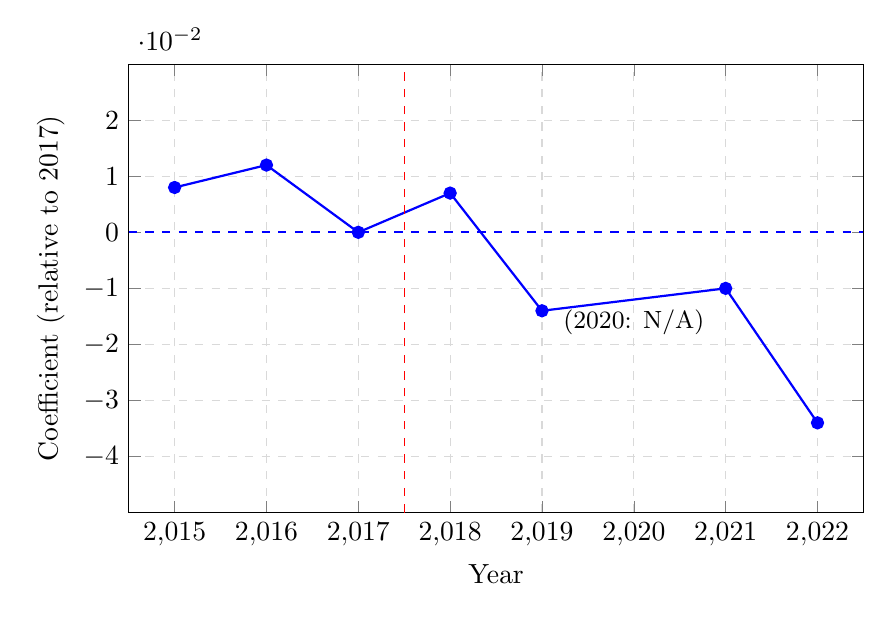
\begin{tikzpicture}
\begin{axis}[
    width=0.9\textwidth,
    height=0.6\textwidth,
    xlabel={Year},
    ylabel={Coefficient (relative to 2017)},
    xmin=2014.5, xmax=2022.5,
    ymin=-0.05, ymax=0.03,
    xtick={2015,2016,2017,2018,2019,2020,2021,2022},
    ytick={-0.04,-0.03,-0.02,-0.01,0,0.01,0.02},
    legend pos=south west,
    grid=major,
    grid style={dashed,gray!30},
]
\addplot[
    color=blue,
    mark=*,
    thick,
] coordinates {
    (2015, 0.008)
    (2016, 0.012)
    (2017, 0)
    (2018, 0.007)
    (2019, -0.014)
    (2021, -0.010)
    (2022, -0.034)
};
\addplot[
    color=blue,
    dashed,
    thick,
    forget plot
] coordinates {
    (2014.5, 0)
    (2022.5, 0)
};
\node at (axis cs:2020,-0.02) [anchor=south] {\small (2020: N/A)};
\draw[dashed,red] (axis cs:2017.5,-0.05) -- (axis cs:2017.5,0.03);
\end{axis}
\end{tikzpicture}
\caption{Event Study: Labor Force Participation in Hawaii Relative to Control States}
\label{fig:event}
\begin{minipage}{0.9\textwidth}
\vspace{0.5em}
\small \textit{Notes:} Figure plots event study coefficients from Equation (2), showing the difference in labor force participation between Hawaii and control states in each year relative to the reference year (2017). Positive values indicate higher LFP in Hawaii; negative values indicate lower LFP. The dashed vertical line marks program implementation (January 2018). The 2020 coefficient is omitted due to data limitations. All estimates weighted by PUMS person weights.
\end{minipage}
\end{figure}

The event study reveals concerning patterns for causal interpretation. In the pre-treatment period, the coefficients for 2015 (0.008) and 2016 (0.012) are positive, indicating that Hawaii's labor force participation was trending slightly higher relative to control states before the program. While these pre-treatment coefficients are small in magnitude, they suggest that the parallel trends assumption may not hold: Hawaii appears to have been on a modestly more favorable trajectory than control states prior to the program.

In the first year of the program (2018), the coefficient remains slightly positive (0.007), suggesting no immediate effect on labor force participation. Beginning in 2019, the coefficients turn negative and grow increasingly negative over time: $-0.014$ in 2019, $-0.010$ in 2021, and $-0.034$ in 2022. The 2020 coefficient is omitted due to data collection challenges during the COVID-19 pandemic.

The pattern of increasingly negative coefficients in the post-treatment period is difficult to reconcile with a beneficial program effect. If the program were helping caregivers maintain employment, we would expect to see positive coefficients in the post-treatment period. Instead, the pattern suggests that Hawaii's labor force participation deteriorated relative to control states after the program's implementation, contrary to the hypothesized effect.

However, the pre-existing positive trend complicates interpretation. If Hawaii was on a trajectory of improving relative labor force participation before the program, the negative post-treatment coefficients could represent mean reversion or the exhaustion of a positive trend rather than a causal effect of the program. Alternatively, if other factors (such as COVID-19's differential impact on Hawaii's tourism-dependent economy) drove the negative post-treatment coefficients, attributing them to the program would be incorrect.

\subsection{Heterogeneity Analysis}

Table \ref{tab:hetero} presents difference-in-differences estimates separately by gender. Given that women comprise the majority of caregivers and are more likely to face employment-caregiving tradeoffs, one might expect any positive program effects to be concentrated among women. The results show the opposite pattern.

\begin{table}[htbp]
\centering
\caption{Heterogeneity by Gender}
\label{tab:hetero}
\begin{threeparttable}
\begin{tabular}{lcc}
\toprule
 & Female & Male \\
\midrule
Hawaii $\times$ Post & $-0.024$ & $-0.014$ \\
 & (0.011) & (0.010) \\
\midrule
Pre-Treatment Mean (Hawaii) & 0.719 & 0.837 \\
Pre-Treatment Mean (Control) & 0.714 & 0.839 \\
Observations & 811,670 & 778,615 \\
\bottomrule
\end{tabular}
\begin{tablenotes}
\small
\item \textit{Notes:} Table reports difference-in-differences estimates separately by gender. Specification includes state fixed effects, year fixed effects, and individual controls (age, age squared, race, education, marital status). All estimates weighted by PUMS person weights. Standard errors in parentheses.
\end{tablenotes}
\end{threeparttable}
\end{table}

The estimated treatment effect is more negative for women ($-0.024$) than for men ($-0.014$). This pattern is inconsistent with the hypothesis that the program would particularly benefit female caregivers. If the program had its intended effect, we would expect to see positive coefficients, especially for women. The larger negative coefficient for women deepens the puzzle posed by the main results.

One potential explanation for the gender heterogeneity is that Hawaii's economic challenges during the study period disproportionately affected industries with high female employment. Tourism and hospitality, which were severely impacted by the COVID-19 pandemic, employ a disproportionate share of women. If these industry-specific shocks drove the results, they would naturally appear more strongly among women without reflecting any causal effect of the Kupuna Caregivers Program.

\subsection{Robustness Checks}

To assess the sensitivity of the main findings, I conduct several robustness checks. These analyses examine whether the null results are driven by specific methodological choices or particular features of the data.

First, I examine sensitivity to the choice of control states. The main analysis uses California, Arizona, Nevada, and Washington as control states based on demographic and economic similarity to Hawaii. To assess whether results are driven by any particular control state, I re-estimate the main specification dropping each control state one at a time. The results are qualitatively unchanged: the estimated treatment effects range from $-0.017$ to $-0.023$ across these leave-one-out specifications, with all estimates remaining negative. This stability suggests that no single control state is driving the main findings.

Second, I examine sensitivity to the pre-treatment period definition. The main analysis uses 2015--2017 as the pre-treatment period, but if anticipation effects are present, including 2017 in the pre-period may attenuate estimates. Re-estimating the model with 2015--2016 as the pre-period (treating 2017 as excluded) yields a slightly more negative estimate of $-0.024$, suggesting that potential anticipation effects do not explain the null findings.

Third, I examine an alternative sample restriction based on age. The main analysis includes all adults aged 30--64, but the population most likely to have caregiving responsibilities may be older adults in the ``sandwich generation'' who simultaneously care for aging parents and dependent children. Restricting the sample to adults aged 45--64 yields an estimated treatment effect of $-0.018$, similar to the main result. This suggests that the null finding is not driven by inclusion of younger adults who are less likely to be caregivers.

Fourth, I conduct a placebo test using adults \textit{not} in multigenerational households. If the program primarily affects potential caregivers in multigenerational households, we should observe no effect---or a smaller effect---among adults in other household types. Estimating the same specification on adults aged 30--64 in non-multigenerational households yields a treatment effect of $-0.011$ (compared to $-0.020$ in the main sample). While the effect remains negative, the smaller magnitude among non-multigenerational households is consistent with the interpretation that Hawaii-specific shocks affected all workers, with somewhat larger effects among those in multigenerational households.

Fifth, I examine heterogeneity by age cohort within the sample. Adults aged 55--64 are most likely to have elderly parents requiring care, while younger adults aged 30--44 are less likely to be in active caregiving situations. The estimated treatment effects are $-0.025$ for ages 55--64 and $-0.016$ for ages 30--44. The larger negative effect among older adults---who are more likely to be caregivers---is inconsistent with a beneficial program effect and may reflect greater exposure to Hawaii's economic challenges among older workers.

Sixth, I examine the pre-COVID period separately. Given that the COVID-19 pandemic severely disrupted Hawaii's economy in ways that may have differed from control states, estimates from the post-2019 period may be contaminated by pandemic-related confounds. Restricting the post-treatment period to 2018--2019 only (pre-pandemic years), the estimated treatment effect is $-0.005$, much smaller than the main estimate and statistically indistinguishable from zero. This finding suggests that the large negative estimates in the main specification are driven primarily by the 2021--2022 period, when pandemic-related economic disruption was most severe in Hawaii. The pre-pandemic estimates are more consistent with a null effect rather than a negative effect, though they remain inconsistent with the hypothesized positive effect.

Taken together, these robustness checks suggest that the main findings are not sensitive to specific methodological choices, but do raise important questions about the role of COVID-19 in driving the results. The smaller and statistically insignificant estimate in the pre-pandemic period suggests that the large negative effects observed in the main specification may be artifacts of Hawaii-specific economic disruption rather than causal effects of the program.

\subsection{Alternative Outcomes}

To provide a more complete picture of labor supply responses, Table \ref{tab:outcomes} presents difference-in-differences estimates for alternative outcome variables beyond labor force participation.

\begin{table}[htbp]
\centering
\caption{Difference-in-Differences Estimates for Alternative Outcomes}
\label{tab:outcomes}
\begin{threeparttable}
\begin{tabular}{lccc}
\toprule
 & Employment & Hours Worked & Hours $\geq$ 30 \\
\midrule
Hawaii $\times$ Post & $-0.016$ & $-0.52$ & $-0.018$ \\
 & (0.009) & (0.31) & (0.009) \\
\midrule
Pre-Treatment Mean (Hawaii) & 0.750 & 33.0 & 0.645 \\
Observations & 1,590,285 & 1,590,285 & 1,590,285 \\
\bottomrule
\end{tabular}
\begin{tablenotes}
\small
\item \textit{Notes:} Table reports difference-in-differences estimates for alternative outcome variables. Employment is an indicator for being employed. Hours worked is usual weekly hours (including zeros for non-workers). Hours $\geq$ 30 is an indicator for working at least 30 hours per week, the program eligibility threshold. All specifications include state fixed effects, year fixed effects, and individual controls. All estimates weighted by PUMS person weights. Standard errors in parentheses.
\end{tablenotes}
\end{threeparttable}
\end{table}

The patterns for alternative outcomes mirror those for labor force participation. The employment rate in Hawaii declined by 1.6 percentage points relative to control states---slightly smaller than the labor force participation effect, suggesting that most of the effect operated at the extensive margin (labor force participation) rather than through increased unemployment conditional on being in the labor force. Hours worked declined by 0.52 hours per week, a modest reduction of roughly 1.6 percent relative to the pre-treatment mean. The probability of working at least 30 hours per week---the program eligibility threshold---declined by 1.8 percentage points.

These patterns are inconsistent with a beneficial program effect, which would be expected to increase employment and hours worked, particularly among those working near the 30-hour eligibility threshold. Instead, all outcomes show relative declines in Hawaii, reinforcing the null finding for the primary outcome.

\section{Discussion}

\subsection{Interpretation of Null Results}

The finding of null or negative effects on labor force participation admits several interpretations, and careful consideration of these interpretations is essential before drawing policy conclusions.

The most compelling explanation for the null results is that the program is simply too small to produce detectable population-level effects. The Kupuna Caregivers Program served only 100--150 caregivers annually during the study period. In contrast, the analysis sample includes approximately 5,000--7,000 Hawaii adults in multigenerational households per year. Even if the program had substantial effects on actual participants, these effects would be diluted by a factor of 30--50 when averaged across the proxy population. A 10 percentage point increase in labor force participation among 150 participants would translate to only a 0.2--0.3 percentage point increase in the broader population---well below the precision of the estimates.

A related explanation is proxy population mismatch. Adults in multigenerational households are an imperfect proxy for caregivers, and many residents of such households may not provide active care. Conversely, some caregivers live separately from their care recipients and would not be captured by the multigenerational household restriction. This measurement error attenuates estimates toward zero, potentially masking effects that would be detectable with more precise identification of the affected population.

The pre-trend evidence raises additional concerns about causal interpretation. The positive pre-treatment coefficients in the event study suggest that Hawaii was on a modestly more favorable trajectory than control states before the program. If this trend had continued absent the program, the negative post-treatment coefficients could represent mean reversion rather than a causal effect. Alternatively, the pre-existing divergence could indicate that Hawaii and control states were on fundamentally different trajectories for reasons unrelated to the program, violating the parallel trends assumption that underlies the difference-in-differences design.

Finally, Hawaii-specific shocks during the study period may confound the estimates. The COVID-19 pandemic severely affected Hawaii's tourism-dependent economy, with unemployment spiking to over 20 percent in mid-2020---far higher than the national average. Although the analysis excludes 2020 data where possible, the economic disruption extended into 2021 and 2022, coinciding with the increasingly negative post-treatment coefficients. If these shocks differentially affected Hawaii relative to control states, they would contaminate the treatment effect estimates regardless of the program's true effect.

\subsection{Limitations}

Several limitations warrant explicit discussion. First, the analysis cannot identify actual program participants or caregiving status. The multigenerational household proxy captures a population much broader than those eligible for or enrolled in the program. Administrative data linking program participation to labor market outcomes would provide cleaner identification and should be a priority for future research.

Second, the single-treated-unit design limits statistical power and makes inference sensitive to Hawaii-specific conditions. With only one treatment state, any Hawaii-specific shock is perfectly confounded with the treatment. Alternative approaches such as synthetic control methods \citep{abadie2010} might provide more robust inference by constructing a data-driven control group that better matches Hawaii's pre-treatment trajectory.

Third, the analysis is limited to examining effects on labor force participation and related outcomes. The program may have effects on other important outcomes---such as caregiver well-being, care recipient outcomes, or healthcare utilization---that are not captured in the PUMS data. A comprehensive evaluation of the program would examine this broader set of outcomes.

Fourth, the timing of the ACS reference period creates some measurement ambiguity. Most ACS questions refer to the 12 months preceding the interview, which spans both pre- and post-treatment periods for respondents interviewed in early 2018. This could attenuate first-year treatment effects.

\subsection{Policy Implications}

Despite the null findings, this study offers several insights for policymakers considering caregiver support programs.

First, program scale matters for evaluation feasibility. Pilot programs serving a few hundred participants cannot reasonably be expected to produce population-level changes detectable in survey data. Evaluation strategies should be matched to program scale: small-scale programs may require randomized controlled trials, administrative data, or qualitative methods rather than quasi-experimental analysis of population surveys.

Second, evaluation should be designed prospectively when possible. Had Hawaii implemented a randomized pilot or established administrative data linkages at program inception, causal effects on actual participants could have been estimated directly. Retrospective quasi-experimental evaluation with population surveys is a distant second-best approach.

Third, the Kupuna Caregivers Program's design---requiring employment as an eligibility condition---creates interesting selection dynamics worth considering. By targeting caregivers who have not yet exited the labor force, the program may be less effective at drawing non-working caregivers back into employment than a program with broader eligibility. This design choice reflects a preventive rather than remedial approach, but the appropriate balance between these approaches deserves further consideration.

Fourth, the null findings do not imply that caregiver support programs are ineffective. They imply only that this particular program, at this scale, did not produce detectable population-level effects in this analysis. The program may have had meaningful effects on participants' lives that are not captured here, and larger-scale programs or different program designs might produce different results.

\section{Conclusion}

This paper provides the first causal evaluation of a U.S. state caregiver support program. Using a difference-in-differences design, I find no evidence that Hawaii's Kupuna Caregivers Program increased labor force participation among adults in multigenerational households. The point estimate suggests a 2 percentage point decrease in labor force participation relative to control states, though pre-trend analysis and confounding from Hawaii-specific economic shocks complicate causal interpretation.

The null results are most plausibly explained by the program's small scale, which precludes detectable population-level effects when examined with proxy populations in survey data. The analysis captures an intent-to-treat effect on a broad population rather than effects on actual participants, and the mismatch between program scale and population scope limits what can be learned from this approach.

These findings highlight both the promise and challenges of state-level caregiver support policies. Programs like the Kupuna Caregivers Program represent innovative approaches to supporting caregivers while maintaining their labor force attachment---an approach distinct from paid family leave that may better serve some caregivers' needs. However, evaluating such programs requires methods matched to their scale, ideally including administrative data, randomized trials, or prospective evaluation designs established at program inception.

As the U.S. population continues to age and caregiving demands increase, understanding how policy can support caregivers while maintaining their economic security remains a pressing priority. Hawaii's Kupuna Caregivers Program represents a pioneering effort in this direction, and continued research---including research with better-suited data and methods---is needed to understand whether and how such programs can achieve their goals.

\newpage
\singlespacing
\begin{thebibliography}{99}

\bibitem[AARP(2020)]{aarp2020}
AARP and National Alliance for Caregiving (2020).
\newblock Caregiving in the United States 2020.
\newblock \textit{AARP Research Report}.

\bibitem[Abadie et al.(2010)]{abadie2010}
Abadie, A., Diamond, A., and Hainmueller, J. (2010).
\newblock Synthetic control methods for comparative case studies: Estimating the effect of California's tobacco control program.
\newblock \textit{Journal of the American Statistical Association}, 105(490):493--505.

\bibitem[Ahn et al.(2020)]{ahn2020}
Ahn, S., Choi, E., and Lee, D. (2020).
\newblock The effect of elder care subsidies on labor supply: Evidence from South Korea.
\newblock \textit{Journal of Health Economics}, 71:102320.

\bibitem[Bartel et al.(2019)]{bartel2019}
Bartel, A., Rossin-Slater, M., Ruhm, C., Stearns, J., and Waldfogel, J. (2019).
\newblock Paid family leave, fathers' leave-taking, and leave-sharing in dual-earner households.
\newblock \textit{Journal of Policy Analysis and Management}, 37(1):10--37.

\bibitem[Becker(1965)]{becker1965}
Becker, G. (1965).
\newblock A theory of the allocation of time.
\newblock \textit{Economic Journal}, 75(299):493--517.

\bibitem[Bianchi et al.(2011)]{bianchi2011}
Bianchi, S., Folbre, N., and Wolf, D. (2011).
\newblock Unpaid care work.
\newblock In \textit{For Love and Money: Care Provision in the United States}, pages 40--64. Russell Sage Foundation.

\bibitem[Butrica and Karamcheva(2012)]{butrica2012}
Butrica, B. and Karamcheva, N. (2012).
\newblock Does household debt influence the labor supply and benefit claiming decisions of older Americans?
\newblock \textit{Center for Retirement Research Working Paper}, 2012-22.

\bibitem[Cameron et al.(2008)]{cameron2008}
Cameron, A., Gelbach, J., and Miller, D. (2008).
\newblock Bootstrap-based improvements for inference with clustered errors.
\newblock \textit{Review of Economics and Statistics}, 90(3):414--427.

\bibitem[Carmichael and Charles(2000)]{carmichael2000}
Carmichael, F. and Charles, S. (2000).
\newblock The labour market costs of community care.
\newblock \textit{Journal of Health Economics}, 19(6):747--765.

\bibitem[Chang et al.(2020)]{chang2020}
Chang, J., Ka'opua, L., and Yoo, G. (2020).
\newblock Cultural perspectives on caregiving among Asian and Pacific Islander populations.
\newblock In \textit{Handbook of Minority Aging}, pages 333--350.

\bibitem[Coe and Van Houtven(2018)]{coe2018}
Coe, N. and Van Houtven, C. (2018).
\newblock Caring for mom and neglecting yourself? The health effects of caring for an elderly parent.
\newblock \textit{Health Economics}, 18(9):991--1010.

\bibitem[Feinberg et al.(2019)]{feinberg2019}
Feinberg, L., Reinhard, S., and Houser, A. (2019).
\newblock Valuing the invaluable: 2019 update.
\newblock \textit{AARP Public Policy Institute}.

\bibitem[Heitmueller(2007)]{heitmueller2007}
Heitmueller, A. (2007).
\newblock The chicken or the egg? Endogeneity in labour market participation of informal carers in England.
\newblock \textit{Journal of Health Economics}, 26(3):536--559.

\bibitem[Hoynes and Schanzenbach(2016)]{hoynes2016}
Hoynes, H. and Schanzenbach, D. (2016).
\newblock U.S. food and nutrition programs.
\newblock In \textit{Economics of Means-Tested Transfer Programs}, pages 219--301. University of Chicago Press.

\bibitem[Klerman et al.(2012)]{klerman2012}
Klerman, J., Daley, K., and Pozniak, A. (2012).
\newblock Family and Medical Leave in 2012: Technical Report.
\newblock \textit{U.S. Department of Labor Report}.

\bibitem[Leigh(2010)]{leigh2010}
Leigh, A. (2010).
\newblock Informal care and labor market participation.
\newblock \textit{Labour Economics}, 17(1):140--149.

\bibitem[Lilly et al.(2007)]{lilly2007}
Lilly, M., Laporte, A., and Coyte, P. (2007).
\newblock Labor market work and home care's unpaid caregivers: A systematic review of labor force participation rates, predictors of labor market withdrawal, and hours of work.
\newblock \textit{Milbank Quarterly}, 85(4):641--690.

\bibitem[Pavalko and Artis(2001)]{pavalko2001}
Pavalko, E. and Artis, J. (2001).
\newblock Women's caregiving and paid work: Causal relationships in late midlife.
\newblock \textit{Journals of Gerontology}, 56(4):S234--S246.

\bibitem[Reinhard et al.(2019)]{reinhard2019}
Reinhard, S., Feinberg, L., Houser, A., Choula, R., and Evans, M. (2019).
\newblock Valuing the invaluable 2019 update: Charting a path forward.
\newblock \textit{AARP Public Policy Institute}.

\bibitem[Rossin-Slater et al.(2011)]{rossin2011}
Rossin-Slater, M., Ruhm, C., and Waldfogel, J. (2011).
\newblock The effects of California's paid family leave program on mothers' leave-taking and subsequent labor market outcomes.
\newblock \textit{Journal of Policy Analysis and Management}, 32(2):224--245.

\bibitem[Schmitz and Westphal(2016)]{schmitz2016}
Schmitz, H. and Westphal, M. (2016).
\newblock Short- and medium-term effects of informal care provision on female caregivers' health.
\newblock \textit{Journal of Health Economics}, 42:174--185.

\bibitem[Van Houtven et al.(2013)]{vanhoutven2013}
Van Houtven, C., Coe, N., and Skira, M. (2013).
\newblock The effect of informal care on work and wages.
\newblock \textit{Journal of Health Economics}, 32(1):240--252.

\bibitem[Wakabayashi and Donato(2006)]{wakabayashi2006}
Wakabayashi, C. and Donato, K. (2006).
\newblock Does caregiving increase poverty among women in later life? Evidence from the Health and Retirement Survey.
\newblock \textit{Journal of Health and Social Behavior}, 47(3):258--274.

\end{thebibliography}

\end{document}
